% GNUPLOT: LaTeX picture with Postscript
\begingroup
  % Encoding inside the plot.  In the header of your document, this encoding
  % should to defined, e.g., by using
  % \usepackage[cp1252,<other encodings>]{inputenc}
  \inputencoding{cp1252}%
  \makeatletter
  \providecommand\color[2][]{%
    \GenericError{(gnuplot) \space\space\space\@spaces}{%
      Package color not loaded in conjunction with
      terminal option `colourtext'%
    }{See the gnuplot documentation for explanation.%
    }{Either use 'blacktext' in gnuplot or load the package
      color.sty in LaTeX.}%
    \renewcommand\color[2][]{}%
  }%
  \providecommand\includegraphics[2][]{%
    \GenericError{(gnuplot) \space\space\space\@spaces}{%
      Package graphicx or graphics not loaded%
    }{See the gnuplot documentation for explanation.%
    }{The gnuplot epslatex terminal needs graphicx.sty or graphics.sty.}%
    \renewcommand\includegraphics[2][]{}%
  }%
  \providecommand\rotatebox[2]{#2}%
  \@ifundefined{ifGPcolor}{%
    \newif\ifGPcolor
    \GPcolorfalse
  }{}%
  \@ifundefined{ifGPblacktext}{%
    \newif\ifGPblacktext
    \GPblacktexttrue
  }{}%
  % define a \g@addto@macro without @ in the name:
  \let\gplgaddtomacro\g@addto@macro
  % define empty templates for all commands taking text:
  \gdef\gplbacktext{}%
  \gdef\gplfronttext{}%
  \makeatother
  \ifGPblacktext
    % no textcolor at all
    \def\colorrgb#1{}%
    \def\colorgray#1{}%
  \else
    % gray or color?
    \ifGPcolor
      \def\colorrgb#1{\color[rgb]{#1}}%
      \def\colorgray#1{\color[gray]{#1}}%
      \expandafter\def\csname LTw\endcsname{\color{white}}%
      \expandafter\def\csname LTb\endcsname{\color{black}}%
      \expandafter\def\csname LTa\endcsname{\color{black}}%
      \expandafter\def\csname LT0\endcsname{\color[rgb]{1,0,0}}%
      \expandafter\def\csname LT1\endcsname{\color[rgb]{0,1,0}}%
      \expandafter\def\csname LT2\endcsname{\color[rgb]{0,0,1}}%
      \expandafter\def\csname LT3\endcsname{\color[rgb]{1,0,1}}%
      \expandafter\def\csname LT4\endcsname{\color[rgb]{0,1,1}}%
      \expandafter\def\csname LT5\endcsname{\color[rgb]{1,1,0}}%
      \expandafter\def\csname LT6\endcsname{\color[rgb]{0,0,0}}%
      \expandafter\def\csname LT7\endcsname{\color[rgb]{1,0.3,0}}%
      \expandafter\def\csname LT8\endcsname{\color[rgb]{0.5,0.5,0.5}}%
    \else
      % gray
      \def\colorrgb#1{\color{black}}%
      \def\colorgray#1{\color[gray]{#1}}%
      \expandafter\def\csname LTw\endcsname{\color{white}}%
      \expandafter\def\csname LTb\endcsname{\color{black}}%
      \expandafter\def\csname LTa\endcsname{\color{black}}%
      \expandafter\def\csname LT0\endcsname{\color{black}}%
      \expandafter\def\csname LT1\endcsname{\color{black}}%
      \expandafter\def\csname LT2\endcsname{\color{black}}%
      \expandafter\def\csname LT3\endcsname{\color{black}}%
      \expandafter\def\csname LT4\endcsname{\color{black}}%
      \expandafter\def\csname LT5\endcsname{\color{black}}%
      \expandafter\def\csname LT6\endcsname{\color{black}}%
      \expandafter\def\csname LT7\endcsname{\color{black}}%
      \expandafter\def\csname LT8\endcsname{\color{black}}%
    \fi
  \fi
    \setlength{\unitlength}{0.0500bp}%
    \ifx\gptboxheight\undefined%
      \newlength{\gptboxheight}%
      \newlength{\gptboxwidth}%
      \newsavebox{\gptboxtext}%
    \fi%
    \setlength{\fboxrule}{0.5pt}%
    \setlength{\fboxsep}{1pt}%
    \definecolor{tbcol}{rgb}{1,1,1}%
\begin{picture}(6802.00,3400.00)%
    \gplgaddtomacro\gplbacktext{%
      \csname LTb\endcsname%%
      \put(-132,220){\makebox(0,0)[r]{\strut{}$-50\%$}}%
      \put(-132,750){\makebox(0,0)[r]{\strut{}$-40\%$}}%
      \put(-132,1280){\makebox(0,0)[r]{\strut{}$-30\%$}}%
      \put(-132,1810){\makebox(0,0)[r]{\strut{}$-20\%$}}%
      \put(-132,2339){\makebox(0,0)[r]{\strut{}$-10\%$}}%
      \put(-132,2869){\makebox(0,0)[r]{\strut{}$0\%$}}%
      \put(-132,3399){\makebox(0,0)[r]{\strut{}$10\%$}}%
      \put(0,0){\makebox(0,0){\strut{}2}}%
      \put(850,0){\makebox(0,0){\strut{}3}}%
      \put(1700,0){\makebox(0,0){\strut{}4}}%
      \put(2550,0){\makebox(0,0){\strut{}5}}%
      \put(3401,0){\makebox(0,0){\strut{}6}}%
      \put(4251,0){\makebox(0,0){\strut{}7}}%
      \put(5101,0){\makebox(0,0){\strut{}8}}%
      \put(5951,0){\makebox(0,0){\strut{}9}}%
      \put(6801,0){\makebox(0,0){\strut{}10}}%
    }%
    \gplgaddtomacro\gplfronttext{%
      \csname LTb\endcsname%%
      \put(-1001,1809){\rotatebox{-270}{\makebox(0,0){\strut{}Average gap to company's solution}}}%
      \put(3400,-330){\makebox(0,0){\strut{}$K$}}%
      \csname LTb\endcsname%%
      \put(5946,2627){\makebox(0,0)[r]{\strut{}600s}}%
      \csname LTb\endcsname%%
      \put(5946,2407){\makebox(0,0)[r]{\strut{}1200s}}%
      \csname LTb\endcsname%%
      \put(5946,2187){\makebox(0,0)[r]{\strut{}1800s}}%
      \csname LTb\endcsname%%
      \put(5946,1967){\makebox(0,0)[r]{\strut{}2400s}}%
      \csname LTb\endcsname%%
      \put(5946,1747){\makebox(0,0)[r]{\strut{}3000s}}%
      \csname LTb\endcsname%%
      \put(5946,1527){\makebox(0,0)[r]{\strut{}3600s}}%
    }%
    \gplbacktext
    \put(0,0){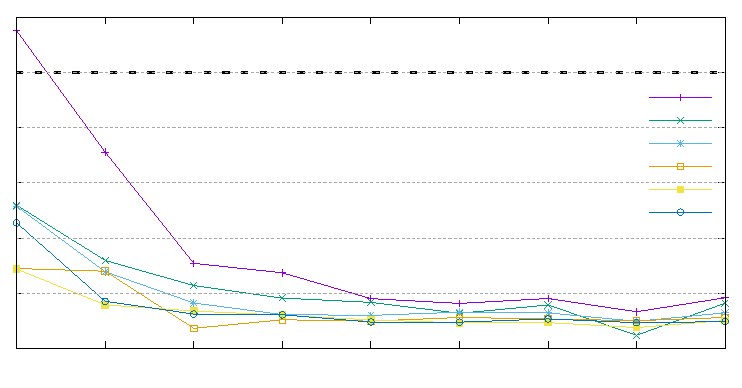
\includegraphics[width={340.10bp},height={170.00bp}]{abkm2020fig7a}}%
    \gplfronttext
  \end{picture}%
\endgroup
